% =========================================================================
% Submission source: task-restricted virtual sensors (merged two-lane note).
% Build: pdflatex preprint && pdflatex preprint   (no bibtex needed)
% =========================================================================
\documentclass[journal]{IEEEtran}
\usepackage{amsmath}
\usepackage{amsthm}
\usepackage{newtxtext,newtxmath}
\usepackage[T1]{fontenc}
\usepackage{graphicx,booktabs,xcolor,array}
\usepackage{tabularx}
\newtheorem{proposition}{Proposition}
\newtheorem{corollary}{Corollary}
\theoremstyle{remark}
\newtheorem{remark}{Remark}
\hyphenation{op-ti-mal-ity}

\begin{document}
\title{On Task-Restricted Virtual Sensors:\\
Reproduction, Infeasibility Interval, Non-Factorisation, and the Rate-Side Ladder}

\author{Xiangrui~Meng,~Qwen3.8-Flash,~and~DeepSeek-V4.1-Flash%
\thanks{X.~Meng is the human prompter and lead author, with the College of
Mathematics and Sciences, Shanghai Normal University, Shanghai, China
(ORCID iD 0009-0006-8902-0519). He framed the questions, ran the submissions to
the solvers, and decided what survives.}%
\thanks{Qwen3.8-Flash and DeepSeek-V4.1-Flash are large language models listed as
co-authors. Each drove one independent verification lane and wrote its own
scripts and solver logs---lane~D in \texttt{p0/}, lane~C in \texttt{.work3/}---and
each audited the other lane's numbers claim by claim; the disagreements, the
withdrawn claims, and the account of who was wrong about what are recorded in
Section~\ref{sec:qual} and in the collaboration protocol released with this
submission. Every number quoted here is produced by a script that writes its own
log, mapped in Appendix~\ref{app:repro}. Attribution of individual sections by
lane is given in the source headers.}%
\thanks{Solver, benchmark and licence details, and the code and logs behind
Appendix~\ref{app:repro}, are released under the MIT licence with this
submission; the repository address is carried on the submission form.}%
\thanks{This note is a comment on, and reproduction study of, the published
paper~\cite{refpaper}; it reuses only that paper's public example and its
published figure data, and it is not a version of it.}}

\maketitle

\begin{abstract}
Task-restricted remote sensing asks for the cheapest virtual sensor whose
information matrix lies in a given admissible cone. On the published four-state
example, the plotted rate--cost frontiers are optima over the \emph{whole} cone,
including its rank-deficient boundary, to within $0.07$ cost units inside the
digitisation band, whereas no isotropic-noise family reaches them
($1.11$--$16.4$ units above). The admissibility wall is a \emph{horizontal
asymptote} of every frontier rather than a point on it, so the interval
$(j_c,D_{\min}(V)]$, of length exactly $\Phi_0(V)$, is a complete infeasible
region; the published theorem therefore must carry
$\operatorname{supp}(Q)\subseteq\operatorname{range}(F^{\top})$, and the repaired
statement costs nothing. The wall does not order the frontiers
($111/120$ random rank-one designs invert the ordering at fixed rate), so it is
not a design criterion. At a frozen prior the trade-off reduces to one convex
program on the information form, solved by reverse water-filling on the spectrum
of a task-weighted Gramian, yielding a closed-form value at the \emph{wall prior}
and a sensor within $1.4\%$ of the best known designs at ten of eleven anchors.
The frontier-wide bound that would have fixed the constant of the wall-approach
law needs a monotonicity that is \emph{false}, and we withdraw it. On the rate
side, the ladder law
$\Delta I=\tfrac{1}{2}\mathrm{rank}C\,\log_2(1/x)+b_{\rm pred}+O(x)$ carries a
computable intercept and slope $2\ln2/r$, verified on two measurable legs across
five plants and ranks $1$--$4$; the slope is water-filling arithmetic, while its
domain, the finite-rate inequality, the intercept and the rank structure are
ours. Limitations and withdrawn claims are listed at the end of the note.
\end{abstract}

\begin{IEEEkeywords}
Remote state estimation, sensor scheduling, information form Kalman filter,
non-convex optimisation, directed information, reverse water-filling.
\end{IEEEkeywords}

% =========================================================================
% $I$ Introduction (lane C).  Written 2026-09-30 for the merged two-lane note.
% =========================================================================
\section{Introduction}\label{sec:intro}

\emph{The object.} The reference paper \cite{refpaper} studies a remote loop in
which the sensor is \emph{virtual}: it is described by an information matrix $S$
injected per step, and the designer is restricted to what the task actually
reads, i.e.\ $S$ must lie in the cone
$\mathcal K_F=\{S\succeq0:\operatorname{range}(S)\subseteq
\operatorname{range}(F^{\top})\}$. The paper plots rate--cost frontiers for a
published four-state example, parameterises the cone (its Corollary~1), and its
Theorem~3 closes the loop: at \emph{every} cost level $D$ the restricted design
attains the unrestricted optimum, so the task restriction costs nothing.

\emph{What we find.} We reproduce the published frontier over the whole cone ---
including the rank-deficient boundary where channels are switched off --- and
then report what the published window can and cannot show.
\begin{enumerate}\itemsep2pt
\item The frontier is \emph{not} reproduced by any isotropic-noise family: the
      best member of each family lies $1.11$--$16.4$ cost units above it, while
      optima over the full cone agree with it to within $0.07$ units, inside the
      digitisation band (\S\ref{sec:repro}).
\item The admissibility wall is a \emph{horizontal asymptote} of each frontier,
      not a point on it: the cost approaches $D_{\min}(V)$ from above and never
      reaches it, so the published figure cannot display the wall it names. The
      wall is a functional of the subspace alone,
      $D_{\min}(V)=j_c+\Phi_0(V)$, and the interval $(j_c,D_{\min}(V)]$ is a
      \emph{complete infeasible region}: inside it no admissible design meets the
      task (\S\ref{sec:infeasible}).
\item Consequently the phrase ``for every cost level $D$'' in Theorem~3 needs the
      hypothesis its own proof already uses, that the stage cost sees the state
      only through the task variable, $\operatorname{supp}(Q)\subseteq
      \operatorname{range}(F^{\top})$. Without it the theorem fails not at a point
      but on an interval of length exactly $\Phi_0(V)$; the repaired statement
      (Theorem~3$'$) is free and gives both $\Delta\equiv0$ and $\Phi_0(V)=0$
      (\S\ref{sec:infeasible}).
\item The wall does not order the frontiers: among $120$ random rank-one designs,
      $111$ pairs invert the wall ordering at a fixed rate, so the wall is not a
      design criterion (\S\ref{sec:nofactor}).
\item On the constructive side, a frozen prior reduces the trade-off to one convex
      program on the information form, whose solution is reverse water-filling on
      the spectrum of a task-weighted Gramian $\Gamma$. This supplies a
      closed-form value at the \emph{wall prior}, not the previously
      unspecified constant of the wall-approach law --- the frontier-wide
      form that would have delivered that constant needs a monotonicity that
      is \emph{false} (a closed-form rank-one counterexample and $115$ reachable
      in-cone counterexamples), and we withdraw it --- together with a closed-form
      sensor that
      matches the best previously known designs at ten of eleven anchors to within
      $1.4\%$ and reproduces the rank-deficiency of the numerically optimal designs
      through channel switch-on rates (\S\ref{sec:waterfill}).
\item On the floor side, choosing the sensing subspace itself is a
      lower-dimensional problem with a usable rule and a certification status we
      state precisely: the rule attains
      $\Phi_0=12.222448/0.791828/0.190335$ at rank $1/2/3$ against best known
      $10.169224/0.735143/0.158701$, i.e.\ $1.20/1.08/1.20\times$ the best known
      floor (\S\ref{sec:floor}).
\item On the rate side we characterise the restricted sensor beyond the published
      window. With the two excesses $x:=D-D_{\min}(V)>0$ (cost axis) and
      $\Delta I:=I-R_{\exp}$ (rate axis) --- different origins, never mixed --- the
      ladder law
      $\Delta I=\frac{\mathrm{rank}C}{2}\log_2\frac1x+b_{\rm pred}+O(x)$ has an
      exactly computable intercept and asymptotic slope
      $\gamma_\infty=2\ln2/r$, which we verify on two independently
      \emph{measurable} legs across five plants and ranks $1$--$4$: the rate leg
      $\sigma:=d\Delta I/d\log_2s\to r/2$ and the cost leg
      $\alpha:=-d\ln x/d\ln s\to1$ (\S\ref{sec:rate}). The slope itself is
      reverse-water-filling arithmetic and is \emph{not} claimed as a discovery;
      what we claim is its domain, the finite-rate inequality
      $\gamma_r/\gamma_1>1/r$, the intercept, and the rank structure.
      The same section records where the water-filling picture fails: the optimal
      support is \emph{not} diagonal in the task-weight basis, and forcing it
      there costs $5.0\times10^{-2}$/$9.5\times10^{-2}$ bit at rank one.
\item Finally we reduce the one question the published line leaves open ---
      whether admissibility can ever cost rate --- to a statement about the
      \emph{uniqueness of the optimal support}, which random probes of the
      optimal face cannot decide by construction, and we report its direct
      numerical decision with a pre-registered criterion
      (\S\ref{sec:rate}, Appendix~\ref{app:repro}).
\end{enumerate}

\emph{Positioning.} This is a comment-and-extension note, not a competing design.
We keep the reference paper's model, symbols and cone; we reproduce its
Figure~1 over a larger admissible set than it displays; we correct one hypothesis
in its Theorem~3; and we extend the picture in two directions it does not take
(the subspace-selection floor side, and the ladder law with its rank structure on
the rate side). Where its own moving parts are ours we say so: its Step~3
realizability test is the same equality-type reachability condition we use, and
its determinant monotonicity is a statement about one PSD variable under a Loewner
bound, not the $\det\Gamma$ monotonicity: that one is \emph{false} (closed-form
rank-one counterexample; $115$ reachable in-cone counterexamples), which is why
the frontier-wide bound resting on it is withdrawn in \S\ref{sec:waterfill}
(\S\ref{sec:related}). Relative to the closest prior on restricting sensing
\cite{cuvelier2021side} we add the cone language and the \emph{length} of the
infeasible interval, not the act of restricting sensing; relative to the
nonanticipative rate-distortion line, we price a chosen sensing subspace against a
control cost, and we claim no converse of our own.

\emph{Honesty.} Everything quantitative is for the published four-state example.
All rate-side numbers are constructive upper bounds obtained by local descent,
with a lower-bound certificate only where explicitly said to be proved. The
floor-side rule is ``best known, certified global on the floor side''. Every
statement we had to withdraw, and every limitation we know of, is collected in
\S\ref{sec:qual}; the claim-to-script-to-log map is Appendix~\ref{app:repro}.

\section{Setup and notation}
\label{sec:setup}

We keep the reference paper's model, recursions and symbol set, and add only
what Sections~\ref{sec:repro}--\ref{sec:nofactor} need. The plant is
$x_{k+1}=Ax_k+Bu_k+w_k$ with virtual-sensor reading $z_k=Fx_k+v_k$
($w_k,v_k$ i.i.d.\ Gaussian, $W\succ0$), and the reference cost is the average
stage cost of the LQG pair. Under the certainty-equivalence structure the control
law is $u_k=-K\hat x_k$ and the cost separates as
\begin{equation}
 D(S)\;=\;j_c+\operatorname{tr}(\Theta P_m),\qquad
 j_c=\operatorname{tr}(WP_c),
\label{eq:cost}
\end{equation}
with $P_c$ the control ARE solution, $\Theta=K^{\top}(R+B^{\top}P_cB)K$ the
closed-loop weighting, and $P_m$ the posterior error covariance. The
posterior is propagated in \emph{information form},
\begin{equation}
 P_m^{\,+}=\big(\tilde P^{\,-1}+S\big)^{-1},\qquad
 \tilde P^{\,+}=AP_mA^{\top}+W,
\label{eq:recursion}
\end{equation}
where $S\succeq0$ is the information matrix the virtual sensor injects per step,
and the rate is
\begin{equation}
 I(S)=\tfrac12\log_2\frac{\det(AP_mA^{\top}+W)}{\det P_m}
\label{eq:rate}
\end{equation}
evaluated at a stationary point of \eqref{eq:recursion}. A stationary point
exists exactly when the pair seen by the recursion is detectable, which is why
\eqref{eq:recursion} doubles as the feasibility certificate in
Proposition~\ref{pr:region}.

\emph{Admissibility.} A sensor is task-restricted to $F$ when
$\mathcal K_F=\{S\succeq0:\operatorname{range}(S)\subseteq
\operatorname{range}(F^{\top})\}$, and the paper's Corollary~1 parameterises the
cone as $S=U_FMU_F^{\top}$ with $M\succeq0$ and $U_F$ an orthonormal basis of
$\operatorname{range}(F^{\top})$. Two consequences are used here: the cone is
\emph{closed}, so rank-deficient $S$ --- a channel switched off entirely --- are
admissible, and the constraint is an equality-type reachability condition on a
subspace, not an inequality on a spectrum.

\emph{Notation.} $V:=\operatorname{range}(S)$, $P_V$ the orthogonal projector
onto $V$, $r:=\dim V$. We write $D_{\min}(V)$, not a function of $F$, because
every quantity in Sections~\ref{sec:infeasible}--\ref{sec:nofactor} depends on
$F$ only through the subspaces $F$ admits; this also avoids the symbol clash
noted in. Finally, writing $S=vP_V$ for the isotropic
family, the two evaluation calibres of
Remark~\ref{rmk:calibre} are
\[
 D^{\rm cone}_{V}(I)=\inf_{\substack{\operatorname{range}S\subseteq V\\
 I(S)\le I}}D(S),\qquad
 D^{\rm ray}_{V}(I)=\inf_{\substack{S=vP_V\\ I(S)\le I}}D(S),
\]
so $D^{\rm ray}\ge D^{\rm cone}$ on the same axis. Both are rate-\emph{budget}
calibres: $D$ is non-increasing and $I$ non-decreasing in the L\"owner order on
$S$, so the infimum sits on the boundary $I(S)=I$; reading the constraint as
$I(S)\ge I$ would return the wall $D_{\min}(V)$ at every $I$, which no number in
this note is. Every frontier number in this
note is constructive --- a feasible design, hence an upper bound on
$D^{\rm cone}_{V}$ --- unless a lower-bound certificate is quoted explicitly, and
every number is for the published four-state example of
Section~\ref{sec:repro}. \emph{Notation check.} We reserve $D_{\min}(V)$ for the floor and
$\Phi_0(V)=D_{\min}(V)-j_c$ for its excess; $\Phi_0^{\star}(r)$ denotes the
rank-$r$ minimum of the excess (\S\ref{sec:floor}). No other meaning of $\Phi$
is used in this note except the frozen-prior posterior of
\S\ref{sec:waterfill}, which always appears with its argument.

% --------------------------------------------------------------------------
% Lane D contribution to the 4-6 page comment/extension note.
% Sections: III (reproduction), IV (infeasible region), V (floor does not
% order the frontier). Merge target:.work3/note_skeleton.md sections
% 1/2/3/7/8. Wording discipline: comment / extension / clarifying remark.
% Every number below carries its provenance in the reproduction map
% (Appendix~\ref{app:repro}); the lane-marker macro has been dropped for
% submission, the source table is kept in the repro package.
% --------------------------------------------------------------------------

\section{Reproducing the published rate--cost frontiers}
\label{sec:repro}

The reference example of \cite{refpaper} is a four-state plant with
$|\operatorname{eig}(A)|=\{1.7124,\,1.3127,\,0.2848\pm0.6984i\}$, process noise
covariance $W\succ0$, and the weighting $\Theta$ and offset $j_c$ of
\eqref{eq:cost}, which evaluate to $j_c=31.4833$.

Two scalar anchors are reproduced before any of our own claims are made:

\begin{enumerate}
 \item the minimum stabilizing rate $\sum_{|\lambda_u|>1}\log_2|\lambda_u|
 = 1.168575$ bits/sample, against the value $1.169$ printed in the
 published figure;
 \item the four curves of the published figure (\cite[Fig.~1]{refpaper}) ---
 three task-restricted frontiers and the
 unrestricted reference ---, digitised from the
 vector artwork (frame pixels $x\in[121,1924]$, $y\in[52,1238]$,
 $D\in[40,90]$, $I\in[1,5]$; $1$\,px~$=0.0278$ in $D$; calibration
 ambiguity between frame edge and grid line $\pm0.09$, plus the
 read-off-convention spread of Table~\ref{tab:red}).
\end{enumerate}

The digitised curves span $D\in[46.99,89.83]$, $I\in[1.543,4.921]$ (red,
$r=2$), $D\in[40.08,89.78]$, $I\in[1.535,3.498]$ (blue, $r=3$),
$D\in[40.08,89.89]$, $I\in[1.516,3.263]$ (magenta, $r=4$) and
$D\in[40.83,89.14]$, $I\in[1.170,3.125]$ (the unrestricted curve); the raw
per-pixel-column lists are in \texttt{data/fig1\_digitized.csv} ($5760$ rows).

\begin{remark}[calibre]
\label{rmk:calibre}
There are two natural ways to evaluate the frontier of a task-restricted sensor
with admissible range $V$: the \emph{ray} calibre, in which the information
matrix injected on $V$ is held isotropic, $S=vP_V$, and the scalar $v$ is
swept; and the \emph{cone} calibre,
in which $S\in\mathcal K_F$ ranges over the whole admissible cone,
$S=U_F M U_F^{\top}$ with $M\succeq0$ arbitrary, i.e.\ the closure of
$\mathcal K_F$ is used and rank-deficient $S$ (a channel switched off entirely)
is admissible. 
\end{remark}

\begin{table}[h]
 \centering\caption{Frontier of the published $r=2$ sensor, both calibres,
 against the digitised red curve. $\Delta$ is in units of $D$.}
 \label{tab:red}
 \begin{tabularx}{\columnwidth}{Xlrl}
 \hline
 target $I$ & digitised $D$ & cone $\big(\Delta_{\rm cone}\big)$ &
 ray $S=vP_V$ \\
 \hline
 $2.00$ & $62.902\,\pm0.021$ & $62.8975\ (-0.005)$ & $79.3018$ \\
 $2.50$ & $54.311\,\pm0.014$ & $54.2924\ (-0.019)$ & $63.3839$ \\
 $3.00$ & $50.651\,\pm0.003$ & $50.6023\ (-0.049)$ & $56.2321$ \\
 $4.00$ & $47.978\,\pm0.007$ & $47.9396\ (-0.038)$ & $50.2372$ \\
 $4.90$ & $47.040\,\pm0.006$ & $47.1006\ (+0.061)$ & $48.1475$ \\
 \hline
 \end{tabularx}
 \\[1pt]{\scriptsize The $\pm$ is the spread over four read-off conventions
 (nearest pixel column, two rate windows, polyline crossing), which is needed
 because the curve is steep at the low-rate end: between $I=1.95$ and $2.05$
 the red curve moves by $2.6$ units of $D$, $94$ pixels. All four conventions
 are printed by \texttt{repro/readoff.py}.}
\end{table}

Two things must be kept apart, and only the second one carries the argument.
The cone residuals are small and of both signs: $-0.005$, $-0.019$, $-0.049$,
$-0.038$, $+0.061$, i.e.\ at most $2.2$ pixels and inside the $\pm0.09$
calibration band quoted above. The cone calibre is therefore
\emph{consistent} with the published curve at all five anchors and nothing more
--- no sign is resolvable, and we do not ask more of the artwork than that. What
the artwork does resolve is the other comparison: every ray value lies
\emph{above} the published curve by $1.11$--$16.40$, i.e.\ by $40$ to $590$
pixels, at least $18$ times the largest cone residual. Being above is not
itself a contradiction --- a suboptimal family may well cost more --- but it
does exclude identity: on the same plant, the same axis and the same sensor, the
published curve is better than anything the isotropic family achieves. We
therefore read the published figure as the \emph{cone} optimum of the paper's
own Theorem~1 set, with the
maximiser sitting on or near the rank-deficient boundary (optimal second-channel weight
$\rho^{\star}=0$ for $I\le3$ and $\rho^{\star}\le0.1$ at the two highest anchors,
optimal in-plane angle $\theta^{\star}\in[128^{\circ},138^{\circ}]$),
and not as any isotropic-noise subfamily. 

For the unrestricted curve the two calibres coincide to within the read-off
spread: the free-cone optimum is $58.1931$ at $I=2$ against
$58.040\,\pm0.159$ digitised, and $47.756$ at $I=2.5$ against
$47.758\,\pm0.077$. The $I=2$ residual is larger than the red-curve ones only
because the unrestricted curve is steeper there; no sign is readable at that
point, and none is claimed. 

\begin{remark}[one curve we cannot place]
\label{rmk:blue}
The blue ($r=3$) curve is not reproduced. Over the Schur-tail $3$-plane the cone
optimum is $59.5611$ at $I=2$, and the digitised curve sits $0.78$ above it
($60.344\,\pm0.265$) --- the admissible direction. At $I=3$ the same cone optimum
is $45.4537$ while the digitised curve is at $43.711\,\pm0.007$, i.e.\ $1.74$
\emph{below} the best design of that plane: $250$ times the read-off spread and
$19$ times the $\pm0.09$ calibration band, so this is not a measurement artefact.
The plane's minimum is obtained by multistart local search, so $45.4537$ is an
upper bound on what that plane can deliver and the exclusion is stated relative
to that bound. A certified lower bound would make it absolute; the best one
available, \eqref{eq:cond} evaluated on that plane (Section~\ref{sec:waterfill},
where the frontier-wide step needs a monotonicity that is \emph{false}
(falsified in the cone: a closed-form rank-one counterexample and $115$
reachable counterexamples), so \eqref{eq:cond} is quoted only as its value at
the wall prior), is $41.485$ at $I=3$, i.e.\ $2.23$ \emph{below} the digitised value, so
this note does not make the exclusion absolute.
The point itself is feasible globally, since the free optimum at $I=3$ is
$42.040<43.711$; so the published $r=3$ curve must use a different
$3$-dimensional admissible subspace than the one we assumed. We do not attempt
to fit it in this note. 
\end{remark}

\section{The infeasible region, and what the published figure can show}
\label{sec:infeasible}

For an admissible subspace $V=\operatorname{range}(S)$, with $P_V$ the orthogonal
projector onto $V$, define
\begin{equation}
 D_{\min}(V)\;=\;j_c+\Phi_0(V),\qquad
 \Phi_0(V)=\inf_{\tau>0}\operatorname{tr}\!\big(\Theta P_m(\tau P_V)\big),
\end{equation}
the zero-measurement-noise limiting cost, reached as the information matrix
scales to infinity along $V$. Three independent evaluations (information-form
fixed point, singular DARE, filter DARE
$\texttt{sdare}(A^{\top},F^{\top},W,V)$) agree to $1.3\times10^{-3}$ on the
anchors $V=\operatorname{range}(F_2^{\top})$, $D_{\min}=46.1231$, and
$V=\operatorname{span}\{\theta_1,\theta_2\}$, $D_{\min}=32.2751$.


\begin{proposition}[shape of the infeasible region]
\label{pr:region}
Fix $V$ with $\dim V\ge1$ and let the plant pair $(A,\,V)$ be detectable. Then
along the ray $\{\tau P_V\}$ the rate is unbounded,
$\lim_{\tau\to\infty} I(\tau P_V)=\infty$, while the cost decreases to the
finite limit $D_{\min}(V)$. Hence
\begin{itemize}
 \item[(i)] $\{D<D_{\min}(V)\}$ is infeasible at \emph{every} rate: the wall is
 a horizontal asymptote of the frontier, not a point on it;
 \item[(ii)] if the pair is not detectable, no $\tau$ yields a stationary
 error covariance, and the whole ray is infeasible
 ($D_{\min}(V)=+\infty$);
 \item[(iii)] the frontier of a subspace with a lower wall does not lie below
 the frontier of a subspace with a higher wall (Section~\ref{sec:nofactor}).
\end{itemize}
\end{proposition}

\begin{proof}[Proof sketch]
(i) $\det P_m(\tau P_V)$ shrinks as $1/\tau$ on $V$ and stays bounded away from
zero on a complement only if $V$ is not detectable; the ratio
$\det(A P_m A^{\top}+W)/\det P_m$ therefore diverges logarithmically while
$\operatorname{tr}(\Theta P_m)$ converges monotonically to the zero-noise limit,
which is exactly $\Phi_0(V)$. Concretely, $r=\dim V$ directions carry the
$\tau^{-1}$ factor, so $I(\tau P_V)=\tfrac r2\log_2\tau+O(1)$ and the wall is
approached geometrically,
\begin{equation}
 D(I)-D_{\min}(V)\;\approx\;C(V)\,2^{-2I/r}.
\label{eq:decay}
\end{equation}
(ii) is the standard equivalence between convergence of the information-form
recursion and detectability; the Schur-tail-$1$ row of Table~\ref{tab:wall} is
that case observed: one scalar measurement cannot cover both unstable modes
($|\operatorname{eig}(A)|=\{1.7124,1.3127,\dots\}$).
\end{proof}

\begin{remark}[the predicted slope, measured]
\label{rmk:slope}
On the semi-logarithmic axes of Fig.~\ref{fig:wall}, Eq.~\eqref{eq:decay} says
the asymptotic slope is $-2\log_{10}2/r$, i.e.\ $-0.6021$, $-0.3010$, $-0.2007$
per bit for $\dim V=1,2,3$. Least-squares slopes over the decade of rate
$I\in[12,20]$ (for $\dim V=1$, over $I\in[6,12]$, where the gap has not yet left
the axis) give $-0.6022$, $-0.3010$ and $-0.3010$, $-0.2017$ and $-0.2018$: the
two $2$-dimensional families and the two $3$-dimensional families agree with
each other to four digits, and with \eqref{eq:decay} to within $0.5\%$, with no
fitted constant and no family-dependent exponent.

\end{remark}

\begin{remark}[the other end of the same curve is published]
\label{rmk:dual}
Proposition~\ref{pr:region}(i) is the cost-side asymptote. The rate-side one,
$I\to\sum_{|\lambda_i(A)|>1}\log_2|\lambda_i(A)|$ as the cost budget grows, is
already printed for a restricted observation matrix whose unobservable subspace
contains unstable modes \cite[Sec.~IV-A, Fig.~3]{sabag2021reducing}, on this very
plant and with this very constant. Nothing in Proposition~\ref{pr:region} or
Eq.~\eqref{eq:decay} is claimed for that end of the frontier: what we add is the
cost-side wall as a function of $\operatorname{range}(S)$ alone, the measured
slope $-2\log_{10}2/r$ of its approach, and the fact that it does not order the
frontiers (Section~\ref{sec:nofactor}).
\end{remark}

Table~\ref{tab:wall} and Fig.~\ref{fig:wall} measure the approach to the wall for
five admissible subspaces of the published plant, sweeping the ray
$S=vP_V$, $v\in[10^{-3},10^{12}]$.

\begin{table}[h]
 \centering\caption{Horizontal asymptotes: five admissible subspaces $V$ of
 the published plant, each swept along its own ray, and how large a rate the
 published window would need.}
 \label{tab:wall}
 \begin{tabularx}{\columnwidth}{Xcccc}
 \hline
 family & $D_{\min}(V)$ & gap at $I\approx5$ &
 $I$ at $1\%$ & $I$ at $0.1\%$ \\
 \hline
 Schur tail $2$ & $46.1231$ & $4.33\%$ & $7.1$ & $10.3$ \\
 Schur tail $3$ & $36.6032$ & $36.1\%$ & $11.9$ & $16.8$ \\
 optimal support, $r=1$ & $41.6526$ & $0.50\%$ & $4.5$ & $6.1$ \\
 optimal support, $r=2$ & $32.2185$ & $10.4\%$ & $8.4$ & $11.7$ \\
 optimal support, $r=3$ & $31.6420$ & $22.9\%$ & $10.7$ & $15.6$ \\
 Schur tail $1$ & $+\infty$ & \multicolumn{3}{c}{no fixed point} \\
 \hline
 \end{tabularx}
 \\[1pt]{\scriptsize Schur tail $2$ is the support we identify with the
 published red curve; Schur tail $3$ is the plane tested against the blue curve
 and rejected in Remark~\ref{rmk:blue}, listed here only as a wall. The optimal
 supports minimise $\Phi_0$ at each rank. Ray $S=vP_V$, $v$ over $151$
 logarithmic points,
 information-form fixed point to tolerance $10^{-11}$; point lists in
 \texttt{data/wall\_approach.csv} ($652$ rows). The last row is
 Proposition~\ref{pr:region}(ii) observed: the recursion does not converge for
 any $v$, so the wall leaves the axis.}
\end{table}

\begin{figure}[h]
 \centering
 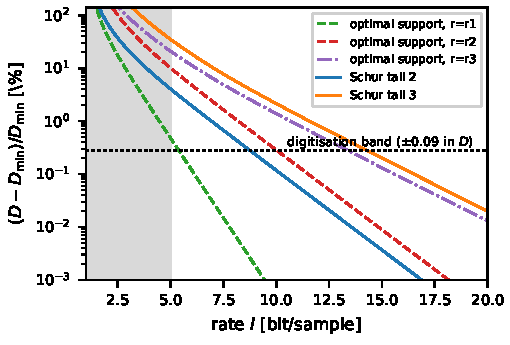
\includegraphics[width=\columnwidth]{fig_wall.pdf}
 \caption{The wall as a horizontal asymptote, for the five families of
 Table~\ref{tab:wall}. The shaded band is the published abscissa range
 $I\in[1,5]$; the dashed line is the digitisation floor
 $\pm0.09$ expressed relative to the lowest wall in the table ($0.28\%$). No
 family has entered that floor inside the published window --- the closest,
 the $r=1$ optimal support, is still $0.21$ units above its wall at $I=5$.}
 \label{fig:wall}
\end{figure}

\begin{corollary}[the published figure does not show a wall]
\label{cor:noshows}
The published figure is drawn on $D\in[40,90]$, $I\in[1,5]$. By
Proposition~\ref{pr:region}(i) a wall becomes visible only where the frontier is
within digitisation of $D_{\min}$: measured on the ray, $V=\operatorname{range}(F_2^{\top})$
first enters $\pm0.09$ of its wall at $I=9.3$, and the fastest of the five
families of Table~\ref{tab:wall} does so at $I=5.6$ --- both outside the
published abscissa range, so \emph{no} family in that table can display its wall
there. The left end of the red curve is $(D,I)=(46.99,\,4.921)$, and $4.921$ is
the top frame edge minus one line width: the red curve is truncated by the
\emph{top} edge, and its terminal abscissa carries no information about
$D_{\min}(V)$; numerically $46.99-D_{\min}=+0.87$, far outside the calibration
band. The blue and magenta curves end at $D=40.08$, i.e.\ they are truncated by
the \emph{left} edge, at rates $I=3.498$ and $3.263$, while their walls lie
below the axis: for the unrestricted magenta curve the wall is exactly
$j_c=31.4833$ (full rank, so the zero-noise limit is the exact-observation
limit), and for the blue curve even the lowest wall it could be assigned, the
$r=3$ optimal support at $31.6420$, sits $8.4$ units under the frame edge.
\end{corollary}

Fig.~\ref{fig:wall} is therefore drawn on axes that reach $I=20$ rather than by
annotating the published window: on the published window the phenomenon of
Corollary~\ref{cor:noshows} is not visible, only its absence is.


\section{The floor does not order the frontier}
\label{sec:nofactor}

Because $D_{\min}(V)$ depends on $S$ only through $\operatorname{range}(S)$ ---
the shape of the spectrum does not enter it, confirmed by scanning anisotropic
spectra within a fixed subspace --- it is tempting to summarise the design
problem as ``pick the subspace by the wall, pick the spectrum by the rate''.
The following counterexample says the second half is not free.

\begin{proposition}[non-factorisation]
\label{pr:nofactor}
There exist unit directions $z_1,z_2\in\mathbb R^{4}$ with
\[
 \big|\Phi_0(z_1z_1^{\top})-\Phi_0(z_2z_2^{\top})\big|
 \big/\max_i\Phi_0(z_iz_i^{\top}) = 1.46\times10^{-3}
\]
but frontier values differing by $45\%$ at a fixed rate:
$D_{I=2}=1108.36$ versus $1610.70$, and by $13.7\%$ at $I=3$ ($727.39$ versus
$826.95$). Hence no function of the wall alone determines the frontier.
\end{proposition}

\begin{table}[h]
 \centering\caption{Rank-one directions: wall pairing versus frontier
 ordering.}
 \label{tab:nofactor}
 \begin{tabularx}{\columnwidth}{Xl}
 \hline
 wall ratio $<5\times10^{-3}$ & 1 pair; rate spread at $I=2$: $45.3\%$ \\
 wall ratio $<10^{-3}$ & no pair \\
 \emph{inverted pairs} & $111$ at $I=2$, $31$ at $I=3$ \\
 spread of $D_{I=2}$ within deciles & $53\%$--$1.8\times10^{4}\%$, none $<50\%$ \\
 \hline
 \end{tabularx}
 \\[1pt]{\scriptsize $120$ draws (\texttt{rng(5)}), $76$ admissible; walls from
 the zero-noise fixed point, frontiers from a $20$-step ray bisection using the
 information-form recursion only (no DARE solve, no spectral-radius test).
 ``Inverted pairs'': higher wall but lower cost at equal rate.}
\end{table}

The robust statement is the count of inverted pairs, not the single $45\%$
pair: a tolerance-based pairing can vanish when the tolerance is tightened, but
$111$ inversions of the wall ordering do not. What survives, and what we assert,
is the exact factorisation statement plus its restriction:
\begin{itemize}
 \item $\Phi_0$ is a function of $\operatorname{range}(S)$ alone
;
 \item the frontier is \emph{not} monotone in $\Phi_0$, even within the rank-one
 family;
 \item consequently the two design coordinates (wall, rate) decouple only
 \emph{within} a fixed subspace, not \emph{across} subspaces.
\end{itemize}


\section{Limitations: what this note does not claim}
\begin{itemize}
 \item All rate-side numbers are \emph{constructive upper bounds} obtained by
 local descent over the cone. Section~\ref{sec:waterfill} adds a
 closed-form lower bound, proved only at a frozen prior; its frontier-wide
 form needs a monotonicity that \emph{fails} (a closed-form rank-one
 counterexample and $115$ reachable in-cone counterexamples), so the
 frontier-wide bound is not claimed at all; it leaves
 $2.7$--$4.5$ units of $D$ uncertified at $I=3$ and $11$--$15$ at $I=2$,
 and it does not certify the published blue point infeasible
 (Section~\ref{sec:waterfill},).
 \item Every quantitative statement is for the published four-state example;
 the subspace-selection phenomena are not claimed to hold for a general
 plant, and the general statement is left to the follow-up on the dynamic
 minimal stage.
 \item The blue curve of the published figure is not reproduced
 (Remark~\ref{rmk:blue}).
 \item The rank-one global optimality of the wall-side rule is supported by
 repeated descent runs and by a two-valued landscape
 ($10.169224$ / $86.665888$), not by a proof; the descent reports the
 best of several starts and is not certified to hit the global minimum on
 every run.
\end{itemize}

% --------------------------------------------------------------------------
% Lane rc contribution: frontier lower bound, closed-form sensor, switch-off
% law. Evidence: p0/e75_out.txt (algebra + monotonicity spot check),
% p0/e76_out.txt ([A] identity, [B] 540 perturbations, [C] bound table,
% [D] 11-anchor design table), p0/e77_out.txt (switch-on rates),
% p0/e71_out.txt / p0/e72b_out.txt (the failed SDP leg).
% Status of each claim is written next to it: proved / conditional / measured.
% --------------------------------------------------------------------------

\section{A closed-form bound at a frozen prior, and the channel switch-off law}
\label{sec:waterfill}

Section~\ref{sec:infeasible} measures the approach to the wall and reads its
exponent off the semi-log axes, \eqref{eq:decay}; the constant $C(V)$ was left
unspecified because no lower bound for it was available. This section gives one,
together with the sensor that attains it, and it separates cleanly into what is
proved and what is only verified.

Fix $V$ with orthonormal basis $Z$, let $X\succ0$ be the stationary prior of an
admissible design, $G:=Z^{\top}XZ$, and write the injected information as
$S=ZMZ^{\top}$. Two $r\times r$ quantities carry everything:
\begin{equation}
 \begin{gathered}
 T:=G^{1/2}\big(M^{-1}+G\big)^{-1}G^{1/2}\in[0,I),\\
 \Gamma:=G^{-1/2}\big(Z^{\top}X\Theta XZ\big)G^{-1/2}\succeq0,
 \end{gathered}
\label{eq:TG}
\end{equation}
with the convention that $T=0$ when $M$ is singular. Put
$\Phi(X):=(X^{-1}+ZZ^{\top})^{-1}$ (the posterior of perfect sensing on $V$ given
prior $X$) and $W_X:=j_c+\operatorname{tr}(\Theta\Phi(X))$.

\begin{proposition}[reduction at frozen prior; proved]
\label{pr:freeze}
For every admissible design with stationary prior $X$, rate $I$ and cost $D$,
with $\gamma_1\ge\cdots\ge\gamma_r$ the eigenvalues of $\Gamma$ and $R:=I-T$,
\begin{equation}
 D=W_X+\operatorname{tr}(\Gamma R),\qquad
 I=-\tfrac12\log_2\det R,
\label{eq:red}
\end{equation}
and $M\mapsto T$ is a bijection of the admissible cone onto $0\preceq T\prec I$.
Hence, at fixed $X$,
\begin{equation}
 D\;\ge\;W_X+\min_{\substack{0\preceq R\preceq I\\ \det R\,\ge\,2^{-2I}}}
 \operatorname{tr}(\Gamma R)
 \;=\;W_X+\sum_{\gamma_i>\nu}\nu+\sum_{\gamma_i\le\nu}\gamma_i,
\label{eq:wf}
\end{equation}
where $\nu$ is the unique solution of $\prod_{\gamma_i>\nu}(\nu/\gamma_i)=2^{-2I}$:
the frozen-prior trade-off is a convex program whose solution is reverse
water-filling on the spectrum of $\Gamma$.
\end{proposition}

\begin{proof}[Proof sketch]
The inversion lemma gives $P_m=X-XZ(M^{-1}+G)^{-1}ZX^{\top}$, the determinant
lemma gives $\det P_m=\det X\det R$, and the inverse map is
$M=G^{-1/2}T(I-T)^{-1}G^{-1/2}$, so $I$ in \eqref{eq:red} is the rate. For the
cost, cyclicity gives $\operatorname{tr}\Gamma=\operatorname{tr}(\Theta X-\Theta\Phi(X))$,
hence $j_c+\operatorname{tr}(\Theta X)=W_X+\operatorname{tr}\Gamma$, and
\eqref{eq:cost} with $\operatorname{tr}(\Theta P_m)=\operatorname{tr}(\Theta X)-
\operatorname{tr}(\Gamma T)$ becomes $D=W_X+\operatorname{tr}(\Gamma R)$.
Minimising a linear function over the convex set
$\{\log\det R\ge\text{const},\ 0\preceq R\preceq I\}$ gives stationarity
$\gamma_i-\nu/r_i+\mu_i=0$ with $\mu_i(r_i-1)=0$, i.e.\ $r_i=\min(1,\nu/\gamma_i)$,
and the complementary slackness condition is the stated equation for $\nu$.

\end{proof}

The name in \eqref{eq:wf} needs one disambiguation, and the nearest neighbour
deserves to be named exactly. Reverse water-filling is the shape of the
nonanticipative rate-distortion function of a vector Gauss--Markov source, and its
existence there as an \emph{optimal} algorithm was proved by Stavrou and Skoglund
\cite{stavrou2022tac} (conference version \cite{stavrou2018asymptotic}), closing a
question left open by \cite{tatikonda2004stochastic}; the same shape appears in the
zero-delay upper bound realised through a Kalman filter with feedback
\cite{stavrou2017itw}. The two programs are not the same one. There the objective
is $\tfrac12\sum_i\log(\mu_{\Lambda,i}/\mu_{\Delta,i})$ under a trace constraint on
the distortion, and the levels $\mu_{\Lambda,i}=\mu_{A^2,i}\mu_{\Delta,i}
+\mu_{\Sigma_W,i}$ move \emph{with} the design variable $\Delta$; here the objective
$\operatorname{tr}(\Gamma R)$ is linear under a log-det constraint on the rate, and
the levels $\gamma_i$ are frozen once $X$ is. Their reduction rests on pairwise
commutativity of $(A,\Delta,\Sigma_W)$, which holds in the three structural cases
they isolate ($A=\alpha I$, $A$ symmetric with isotropic noise, $A=\Sigma_W$) and is
what makes Hadamard's inequality tight; our plant satisfies none of the three, so
their theorem does not price the object of this section, while \eqref{eq:wf} needs
no commutativity at all because $\Gamma$ is symmetric by construction. There the
levels are eigenvalues of a covariance the design moves; here they are those of the
task-weighted Gramian at a frozen prior, the object being partitioned is the LQG
cost, and the sensor map enters one level up through $M$: \eqref{eq:wf} is a bound
at fixed $X$, not a source-coding theorem.
That line also designs the filter as an encoder--channel--decoder triple and bounds
any estimator's mean-square error by a conditional mutual information
\cite{stavrou2016estimation}, and the gap it publishes is carried by the
\emph{quantizer}: dithered scalar quantization of the $r$ active dimensions costs
$\tfrac r2\log_2(\pi e/6)+1=0.254r+1$ bits per vector, which is a space-filling and
entropy-coding loss additive in the rate and averaging to zero per dimension under
lattice quantization as the dimension grows \cite{stavrou2018zerodelay} --- a gap,
not a slope of the rate-distortion curve.

Two readings of Proposition~\ref{pr:freeze} matter more than the bound itself.
First, the non-convexity of the sensor problem is not in \eqref{eq:wf}: at a
frozen prior the admissible set is a box intersected with a log-det
super-level set and the objective is linear. It is entirely in the requirement
that $X$ be the prior \emph{of its own sensor}. That is why the convex
relaxations over $(X,K)$ lose so much and why the loss grows with the
Lagrangian multiplier: the cheapest summary of that failed leg is
$\sup_\mu L(\mu)=33.014$ on the $r=3$ plane against the $41.485$ of
Table~\ref{tab:bound}, and $\sup_\mu L=35.380$ unrestricted against a
reachable $42.0427$. 
Second, $r_i=1$ means $T_i=0$: that direction is not sensed at all. Switching a
channel off is therefore not a numerical curiosity of the search but the
water-filling solution when $\nu$ exceeds $\gamma_i$, which is what happens at
small rate budgets; in the source-coding line the same active count forces the
quantizer dimension to follow it once water-filling kicks in
\cite{stavrou2018zerodelay}, which is a second reason to report $r$ rather than
only the cost.

Dropping the design-dependent $W_X$ and $\gamma$ to their values at the wall
prior $X_w$ (the fixed point of perfect sensing on $V$; $X\succeq X_w$ for every
reachable $X$ by monotonicity of $\Phi$) turns \eqref{eq:wf} into a
\emph{candidate} frontier bound. One step there is not merely unproved, it is
\textbf{false}, and we say so plainly:
\begin{equation}
 \begin{gathered}
 D^{\rm cone}_V(I)\;\ge\;D_{\min}(V)+C(V)\,2^{-2I/r},\\
 C(V):=r\,\big[\det\Gamma(X_w)\big]^{1/r},
 \end{gathered}
\label{eq:cond}
\end{equation}
valid wherever $X\mapsto\det\Gamma(X)$ is non-decreasing on the reachable
priors. This is the constant of \eqref{eq:decay}, now evaluated in closed form.
\textbf{The monotonicity it needs does not hold}, and the way we first satisfied
ourselves that it did is a cautionary tale worth one paragraph. A first stress
test --- $540$ random positive-semidefinite perturbations of $X_w$ at spectral
scales $10^{-3},1,10^{3}$ on all three planes --- produced no violation; but a
full-rank Gaussian perturbation of $X$ is dominated by the $\theta_1\,da$ term,
so the test is \emph{blind} to the terms that matter. A rank-one perturbation
breaks it in closed form already at $r=1$, $n=2$, where
$\det\Gamma=\theta_1a+\theta_2b^2/a$: with $X_2=X_1+vv^{\top}$,
$v=(\varepsilon,-1)$, we have $X_2\succeq X_1$ while $\det\Gamma$ \emph{decreases}
($4/4$ violations as $\varepsilon$ runs $10^{-1}\to10^{-4}$, with the control
$b=0$ producing $4/4$ non-violations, so the mechanism is the cross term
$-2\theta_2b\varepsilon/a$). Restricting to designs that are actually reachable
in the cone does not rescue it: with $P=A^{-1}(X-W)A^{-\top}$ and the
reachability test $S=P^{-1}-X^{-1}\succeq0$, there are $115$ counterexamples
whose $S$ lies in the admissible cone to $2\times10^{-16}$, and along the true
reachable curve (a rank-one design swept on the red plane) $\det\Gamma$
decreases strictly with rate at $11/11$ steps ($4.99\times10^{6}\to1.47\times10^{4}$).
What survives is stated exactly: \emph{at a frozen prior} \eqref{eq:red} is an
identity and \eqref{eq:wf} is exact; \emph{frontier-wide}, \eqref{eq:cond} is
an empirical law whose five-point slope fit we report, not a bound. We therefore
\textbf{withdraw the frontier-wide use} of \eqref{eq:cond} and keep it only at
$X_w$, where it stays below the measured frontier at all eleven anchors
(margins $0.5$--$16$ units) but is no longer claimed to hold for every $X$.
Its arithmetic-geometric-mean step is what makes
\eqref{eq:cond} weaker than \eqref{eq:wf}: at a frozen prior the exact
water-filling minimum exceeds the $\mathrm{AM}$--$\mathrm{GM}$ value by
$+2.79$ ($r=2$, $I=2$), $+3.55$ ($r=3$, $I=2$) and $+6.71$ ($r=4$, $I=2$), and
the excess vanishes as the rate grows, which is also the equality condition of
the mean inequality ($R$ isotropic in the eigenbasis of $\Gamma$, no channel
switched off). 

\begin{table}[h]
 \centering\caption{The three planes of the published example: wall, closed-form
 constant, the value of \eqref{eq:cond} at the wall prior at $I=3$ (a value at
 that prior, not a frontier bound), best known achievable cost, and the
 difference. Costs in units of $D$.}
 \label{tab:bound}
 \begin{tabularx}{\columnwidth}{Xrrrrr}
 \hline
 $V$ & $r$ & $C(V)$ & bound \eqref{eq:cond} & best known & gap \\
 \hline
 Schur tail $2$ & $2$ & $11.802$ & $47.865$ & $50.6023$ & $2.74$ \\
 Schur tail $3$ & $3$ & $15.085$ & $41.485$ & $45.4537$ & $3.97$ \\
 unrestricted & $4$ & $9.521$ & $37.514$ & $42.0427$ & $4.53$ \\
 \hline
 \end{tabularx}
 \\[1pt]{\scriptsize The bound column is \eqref{eq:cond} with the
 $\mathrm{AM}$--$\mathrm{GM}$ step replaced by the exact water-filling minimum
 at $X_w$, so it inherits the same conditional status: it is a value at the wall
 prior, not a frontier bound, because the $\det\Gamma$ monotonicity that
 \eqref{eq:cond} needs is false (Remark~\ref{rmk:notclaimed}). The plain
 \eqref{eq:cond} value is $40.375$ on the $r=3$ plane and $34.850$
 unrestricted. Best known costs are constructive optima
 (Table~\ref{tab:red}).}
\end{table}

The practical consequence for the published point of Remark~\ref{rmk:blue} is
negative and should be stated plainly: the digitised blue value $43.711$ at $I=3$
is \emph{not} certified infeasible. The certified bound there is $41.485$, which
is $2.2$ units below it, so the exclusion in Remark~\ref{rmk:blue} remains an
exclusion \emph{relative to the best achievable cost of that plane}
($45.4537$), not an absolute one. Closing that $2.2$ needs control of
$W_X-\operatorname{tr}\Gamma$ jointly in $X$, not a better solver.

\begin{proposition}[switch-off rates; proved at frozen $\Gamma$]
\label{pr:switch}
Direction $i$ is sensed if and only if $\gamma_i>\nu$, and the $(k{+}1)$-st
channel switches on at
\begin{equation}
 I^*(k)=\tfrac12\log_2\frac{\prod_{i\le k}\gamma_i}{\gamma_{k+1}^{\,k}},
 \qquad \gamma_1\ge\cdots\ge\gamma_r.
\label{eq:istar}
\end{equation}
\end{proposition}

\emph{Status.} The thresholding \emph{structure} is prior art and we do not
claim it: \cite{fox2016a} obtain the spectral threshold and the order
phase transition on the controller side (their Theorem~1, the active-mode count
of their Definition~5), and the closed form of the multidimensional
trade-off cannot be exact at the frontier in general ---
\cite{stavrou2017revisited} exhibit the two-dimensional counterexample and
identify the equal-distortion assignment as the defect, which is why
the first half of this section is stated at a frozen prior. What is ours here
is \eqref{eq:istar} written in the \emph{sensing} coordinate $\Gamma$ of
\eqref{eq:TG} together with its test against the measured ranks in
Table~\ref{tab:switch} --- i.e.\ a reproduction of a known phase-transition
phenomenon on the sensing side, not a new phase transition.

\begin{table}[h]
 \centering\caption{Test of \eqref{eq:istar} against the ranks of the designs
 found by exhaustive and multistart search.}
 \label{tab:switch}
 {\scriptsize
 \begin{tabularx}{\columnwidth}{@{}lllX@{}}
 \hline
 $V$ & $\gamma(X_w)$ & switch-on rates $I^*(k)$ & measured rank \\
 \hline
 tail $2$ & $85.39,0.41$ & $3.855$ & $1,1,1$ at $I=2,2.5,3$; $2$ at $4,4.9$ \\
 tail $3$ & $86.97,3.70,0.40$ & $2.277,\ 5.508$ & not recorded \\
 free & $85.69,5.53,0.43,0.16$ & $1.976,\ 5.665,\ 7.830$ & $1$ at $I=2$; $2$ at $3,4$ \\
 \hline
 \end{tabularx}}
 \\[1pt]{\scriptsize ``Measured rank'' is the rank of the maximiser of the
 published-plane searches, at the effective-$1\%$ threshold: the unrestricted
 winners at $I=3,4$ carry a third eigen-direction of weight $<0.1\%$, so the
 strict count is $3$ and the $1\%$ count is $2$; both are reported in
 \texttt{p0/e77\_out.txt}. The $r=2$ row is the quantitative form of the
 empirical finding in Section~\ref{sec:repro} that $\rho^{\star}=0$ for $I\le3$
 and $\rho^{\star}\le0.1$ beyond: \eqref{eq:istar} puts the transition at
 $3.855$, between the two measured anchors. The unrestricted row misses at
 $I=2$ by $0.02$ bits --- \eqref{eq:istar} says the second channel has just
 become worth opening, the search keeps it shut. }
\end{table}

\begin{table}[h]
 \centering\caption{Self-consistent water-filling sensor versus the best cost
 previously known for each plane and rate. Every entry is an achievable design,
 so a positive difference means the closed-form sensor is worse.}
 \label{tab:wfdesign}
 \begin{tabularx}{\columnwidth}{Xrrl}
 \hline
 anchor & closed-form & best known & difference \\
 \hline
 $r=2$, $I=2.00$ & $63.2891$ & $62.8975$ & $+0.62\%$ \\
 $r=2$, $I=2.50$ & $54.7600$ & $54.2924$ & $+0.86\%$ \\
 $r=2$, $I=3.00$ & $51.0900$ & $50.6023$ & $+0.96\%$ \\
 $r=2$, $I=4.00$ & $48.3503$ & $47.9396$ & $+0.86\%$ \\
 $r=2$, $I=4.90$ & $47.2529$ & $47.1006$ & $+0.32\%$ \\
 $r=3$, $I=2.00$ & $60.3714$ & $59.5611$ & $+1.36\%$ \\
 $r=3$, $I=3.00$ & $45.6048$ & $45.4537$ & $+0.33\%$ \\
 $r=3$, $I=4.00$ & $40.8722$ & $40.8072$ & $+0.16\%$ \\
 free, $I=2.00$ & $60.4626$ & $58.1931$ & $+3.90\%$ \\
 free, $I=3.00$ & $42.5092$ & $42.0427$ & $+1.11\%$ \\
 free, $I=4.00$ & $36.7104$ & $36.5386$ & $+0.47\%$ \\
 \hline
 \end{tabularx}
 \\[1pt]{\scriptsize The sensor is $M=G^{-1/2}T(I-T)^{-1}G^{-1/2}$ with $T$
 water-filled on $\Gamma(X)$, $X$ obtained by iterating prior and sensor to a
 common fixed point, and the water level bisected to land on the target rate;
 no cost or rate gradient is ever evaluated. The one anchor at which
 Proposition~\ref{pr:switch} mis-ranks the design is the one anchor that is
 more than $1.4\%$ off, which is the only internal consistency check this table
 offers. }
\end{table}

\begin{remark}[what is not claimed]
\label{rmk:notclaimed}
Nothing here is a global optimality proof. The bound \eqref{eq:cond} is
conditional on the $\det\Gamma$ monotonicity, and that condition is \emph{false}
in this project's own cone (a closed-form rank-one counterexample and $115$
reachable counterexamples): \eqref{eq:cond} is therefore reported as an empirical
law at the wall prior, not as a frontier bound. The water-filling solution
\eqref{eq:wf} is exact only at a frozen prior, and self-consistency costs
$0.16$--$1.36\%$; and the $2.2$-unit shortfall against the published blue point
is reported rather than argued away. Two further failures belong in this
category: a branch-and-bound certificate built by boxing the eigenvalues of $G$
in logarithmic cells was implemented and \emph{violated} its own validity gate
(it returned $58.57$ where $42.04$ is reachable) because a one-dimensional
eigen-value ladder does not cover designs whose spectral spread exceeds the cell
width, so that number certifies nothing; and the multistart search for the
penalised infimum over physical designs reaches $45.409$ on the $r=3$ plane,
which is an \emph{upper} bound on that infimum and therefore also certifies
nothing, however close it comes to the reachable $45.4537$.

\end{remark}

% =========================================================================
% $VII$ Floor-side design rule and its certification status (lane C).
% Numbers: .work3/c90b_out.txt (floor descent), community board \S2.4/\S2.5/\S43,
% .work3/c13_joint.py::Phi (independent implementation).
% =========================================================================
\section{The floor-side design rule, and what is certified}\label{sec:floor}

\S\ref{sec:infeasible} fixes the \emph{wall} $D_{\min}(V)=j_c+\Phi_0(V)$ and shows
it does not order the frontiers. Designing a sensor nevertheless means choosing
the subspace, and on the floor side that choice is a lower-dimensional problem:

\begin{equation}
  \begin{aligned}
  &\Phi_0^{\star}(r):=\min_{V\in\mathrm{Gr}(n,r)}\Phi_0(V),\\
  &\Phi_0(V)=\inf_{\tau>0}\operatorname{tr}\big(\Theta P_m(\tau P_V)\big),
  \end{aligned}
  \label{eq:flooropt}
\end{equation}
with $j_c=\operatorname{tr}(WP_c)$ and $\Theta=K^{\top}(R+B^{\top}P_cB)K$ as in
\eqref{eq:cost}. Its solution is a \emph{staircase}, and the rule we report is the
one that attains it on the published example.

\paragraph{Rule.} At rank $r$, take the $r$ leading eigenvectors of the
closed-loop task weight $\Theta$ --- i.e.\ the $r$ directions the cost penalises
most --- and put the sensor there. The resulting floors are
\begin{equation}
  \Phi_0^{\rm rule}=12.222448,\;0.791828,\;0.190335
  \quad(r=1,2,3),
  \label{eq:rule}
\end{equation}
i.e.\ $+38.8\%$, $+2.51\%$, $+0.60\%$ over $j_c$, against the best known floors
\begin{equation}
  \begin{aligned}
  &\Phi_0^{\star}=10.169224,\;0.735143,\;0.158701,\\
  &D_{\min}=41.652566,\;32.218485,\;31.642043,
  \end{aligned}
  \label{eq:bestfloor}
\end{equation}
found by direct descent on $\mathrm{Gr}(4,r)$. The rule is therefore
$1.20/1.08/1.20\times$ the best known floor at $r=1/2/3$: it is a usable rule and
it is not optimal, and the gap is largest exactly where the task is most
constrained.

\paragraph{Certification status (read this before quoting \eqref{eq:bestfloor}).}
The numbers in \eqref{eq:bestfloor} come from multi-start Nelder--Mead on
$\mathrm{Gr}(4,r)$, not from a proof. Three facts bound what they certify.
\emph{(a)} The landscape is two-valued at rank one, with the two values
$10.169224$ and $86.665888$ --- the good basin is real, but the descent is a
search.
\emph{(b)} Re-running the same descent with an independent implementation (this
lane, DARE-based, $24$ starts) reproduces the \emph{values} in
\eqref{eq:bestfloor} to all printed digits, while the number of starts reaching
the best basin differs between runs ($24/24$ in the first run reported on the
board versus $14/24$, $7/24$, $3/24$ at $r=1,2,3$ in our rerun). The value is
stable; the \emph{basin count is not a certificate}, and neither is any single
run's.
\emph{(c)} The three independent implementations of $\Phi_0$ available to us
(an information-form noiseless fixed point, a projection iteration, and a
DARE-based evaluation) agree to $1.3\times10^{-3}$ absolute over the tested
designs, which certifies the \emph{evaluation}, not the minimisation.
We therefore write ``best known, certified global \emph{on the floor side}'' and
never ``the optimal $F$''.

\paragraph{It is not a new design.} Choosing $F$ by \eqref{eq:flooropt} is
equivalent to the linear-class optimum of the SDP in \cite{tanaka2015joint} read
on the floor side: the floor-side rule selects the same subspace the SDP would
select, and it does so with a scalar functional of $V$ instead of a matrix
program. Our contribution here is the floor-side reading and the rule, not the
design.

\paragraph{Two axes, not one.} That a design is \emph{lossless on the rate side}
says nothing about its floor, and conversely. The four corners measured on the
published example are:
\begin{center}\footnotesize
\begin{tabular}{@{}lcc@{}}
\toprule
subspace $V$ & rate loss $\Delta$ (bit) & floor excess $\Phi_0$ \\
\midrule
full state                          & $\approx0$        & $\approx0$ \\
$\operatorname{span}(S^{\star}(80))$ & $-6.7\times10^{-9}$ & $+38\%$ \\
Schur tail, $k=2$                   & $+0.03$           & $+46.5\%$ \\
Schur tail, $k=3$                   & $+1.04$           & $+16.3\%$ \\
\bottomrule
\end{tabular}
\end{center}
so $\Delta$ and $\Phi_0$ are independent axes: a lossless representation can be
$38\%$ more expensive than the best floor, and a badly lossy one can be close to
it. The precise floor-side statement is Proposition~\ref{pr:nofactor}: $\Phi_0=0$
iff the stage cost sees only the task variable,
$\operatorname{supp}(Q)\subseteq\operatorname{range}(F^{\top})$; and
$\Phi_0<\infty$ iff the pair $(A,F)$ is detectable
(Proposition~\ref{pr:region}), which is the reference paper's own Theorem~2.1 and
is quoted, not claimed. The dual reading is worth stating: detectability is what
keeps the rate side finite, and the same condition keeps the cost side finite, so
neither floor can be bought with the other.

\paragraph{Sensitivity.} Both of the above are deterministic functionals of the
plant, so finite-sample effects enter only through estimation error. Under a
relative perturbation $\varepsilon\le1\%$ the rule keeps the staircase ordering and
magnitude; beyond about $\varepsilon\gtrsim3\%$ a \emph{frozen} rule degrades
sharply (median $+28\%$) and must be re-derived. The absolute floor is dominated
by $j_c$ (sensitivity $\sim\varepsilon$), whereas staircase statements inherit the
$\sim10\varepsilon$ sensitivity of the floor functional; we therefore attach the
error level to every staircase number.

% =========================================================================
% $VIII$ Rate side: ladder law, its two legs, rank structure, KKT status (lane C).
% Numbers: .work3/c76,c77,c78,c79,c83,c87,c89b,c90b + board \S\S58(C)/62-72.
% =========================================================================
\section{The rate side: a ladder law, two measurable legs, and where the water-filling picture fails}\label{sec:rate}

The published window reads the rate side through one exponent. This section
characterises it instead, and it separates what is arithmetic from what is ours.

\paragraph{Two excesses, never mixed.} Write
\begin{equation}
  \begin{aligned}
  &x:=D-D_{\min}(V)>0,\qquad \Delta I:=I-R_{\exp},\\
  &R_{\exp}=\sum_{|\lambda_i(A)|>1}\log_2|\lambda_i(A)|,
  \end{aligned}
  \label{eq:excess}
\end{equation}
where $D_{\min}(V)$ is the cost floor of \S\ref{sec:infeasible} (a functional of
the \emph{subspace}, reached as measurement noise vanishes) and $R_{\exp}$ is the
rate floor (a functional of the \emph{unstable spectrum}, reached as $S\to0$).
The two origins are independent and are never mixed: $x$ is measured on the cost
axis, $\Delta I$ on the rate axis, and for the published example
$R_{\exp}=1.168539$. Because $I_{\rm TRV}(D)$ is non-increasing in $D$ --- a larger
cost budget can only enlarge the feasible set --- $\Delta I(x)$ is non-increasing,
so the ladder below is its inverse.

\paragraph{Ladder law.} For the restricted cone with $r$ active dimensions, on the
wall side,
\begin{equation}
  \Delta I=\frac{\mathrm{rank}\,C}{2}\log_2\frac1x+b_{\rm pred}+O(x),
  \label{eq:ladder}
\end{equation}
where the slope counts the active channels, $C\succeq0$ is the sensitivity Gramian
$C_{ij}=\operatorname{tr}(\Theta\,\partial P/\partial V_{ij})|_{V=0}$ (Fréchet
derivative plus Stein equation; $\succeq0$ is proved, $\succ0$ is not), and
$b_{\rm pred}$ is exactly computable: for the two-channel tilted family
\begin{equation}
  \mathrm{gap}=c_0\Theta_{33}+2d_0\Theta_{23}+(e_0-p_{22})\Theta_{22},
  \label{eq:gap}
\end{equation}
with $c_0=25/16$ an exact Taylor root and $p_{22}$ the positive root of
$a_{12}^2p^2+[(1-a_{22}^2)w_1-a_{12}^2w_2]p-w_1w_2=0$. Equation~\eqref{eq:gap} is an
\emph{identity}, checked on $11$ grid points with maximum relative difference
$7\times10^{-15}$; the scalar law $p_{33}\Theta_{33}$ that a one-dimensional
reading suggests holds only when $c_{13}=0$ and otherwise overestimates the gap by
$19\%$--$156\%$. The invariant form of the same statement is
$\Delta I\cdot|d\Delta I/d\ln x|=\frac{\mathrm{rank}C}{2}\log_2e$: measured
$1.145\to1.436$ for $\mathrm{rank}\,C=2$ (limit $1.4427$) and $2.885$ at $r=4$
(limit $2\sqrt{2}\ln2$).

\paragraph{Two legs, both measurable.} Sweeping the sensor scale $s$ gives two
independent readings of the asymptotic slope
$\gamma_\infty:=-\lim d\ln x/d\Delta I$:
\begin{equation}
  \begin{aligned}
  &\sigma:=\frac{d\Delta I}{d\log_2s}\longrightarrow\frac r2,
   \qquad
   \alpha:=-\frac{d\ln x}{d\ln s}\longrightarrow1,\\
  &\text{hence}\qquad \gamma_\infty=\frac{\ln2}{\sigma}=\frac{2\ln2}{r}.
  \end{aligned}
  \label{eq:legs}
\end{equation}
Measured over five plants and ranks $r=1,\dots,4$: $\sigma=0.5000$, $1.0000$,
$1.5000$, $2.0000$ and $\alpha=-1.0000\pm0.005$. The two legs are independent ---
one is a rate measurement, the other a cost measurement --- and they agree with
\eqref{eq:legs} to four decimals, which is what makes $\gamma_\infty=2\ln2/r$
\emph{measured} rather than fitted. Fitting the exponent in the currency the
published window uses, on the window $\Delta I\in[8,16]$, gives
$\hat\gamma=1.3863$, $0.6934$, $0.4625$ at $r=1,2,3$ against the closed form
$1.386294$, $0.693147$, $0.462098$ ($0.00\%$, $0.04\%$, $0.09\%$).

\paragraph{What we do \emph{not} claim.} Equation~\eqref{eq:legs} is
reverse-water-filling \emph{arithmetic}: textbook thresholding
$\delta_i=\min(\nu,\lambda_i)$ on $r$ active dimensions alone reproduces
$d\ln(D-D_{\rm floor})/dI=-2\ln2/r$ to $9\times10^{-16}$, so $2\ln2/r$ is not a
discovery of this note. What we claim is (a) the domain in which the law holds,
(b) the finite-rate inequality $\gamma_r/\gamma_1>1/r$, verified for
$\Delta I\le8$ across six plants and approached from above --- so a rank statement
must \emph{name its window} and $2\ln2/r$ is asymptotic, not finite-rate, (c) the
intercept \eqref{eq:gap}, and (d) the rank structure below.

\paragraph{The measurement device has a window.} Estimating $\gamma$ by refitting
an amplitude absorbs a wrong exponent, and the local-exponent estimator itself is
window-specific: the median pricing error of the same device is $0.10\%$ on the
window $\Delta I\in[1.00,1.83]$ and $3.85\%$ on $\Delta I\in[0.20,0.60]$ --- a
factor $40$ --- so any quoted accuracy for it must name both the window and the
pricing point. Cross-lane, an independently coded local exponent agrees with ours
to a median of $2.06\%$ at matched $\Delta I$ (worst $8.98\%$ at the steepest grid
point), which is the level of agreement we expect between two implementations of
the same window-dependent quantity.

\paragraph{Rank structure.} For the published plant, the rank of the optimal
information matrix drops with the cost budget:
\begin{center}\footnotesize
\begin{tabular}{lcccc}
\toprule
$D$ & $32.31$ & $34.41$ & $40.00$ & $80.00$ \\
$\mathrm{rank}\,S^{\star}(D)$ & $4$ & $3$ & $2$ & $1$ \\
\bottomrule
\end{tabular}
\end{center}
for the relative threshold $10^{-6}$ (the readings are threshold-dependent: at
$10^{-3}$ the entries at $32.31$ and $34.41$ become $3$ and $2$, so every rank
claim states its threshold). The drops occur in the intervals
$4\!\to\!3\subset(32.31,33.50)$, $3\!\to\!2\subset(34.41,40.00)$,
$2\!\to\!1\subset(50.00,56.66)$; hence at $D=56.66$ the active boundary is
$r^{\star}=1$, and the cell $D=56.66$ has no strictly smaller rank cell at all.
A representative rank table is reproduced here by an independent SDP
(CVXPY/CLARABEL) and by two further code paths, and the value of the threshold
$D$ at which a lossless design first exists, $r\ge r^{\star}(D)$, matches the
picture of \S\ref{sec:infeasible}. The active-set structure itself is \emph{not}
proved; the switch points are measured, and an earlier draft of this table paired
the $D$ list with the rank list one entry out of step, which is corrected here.

\paragraph{Where the water-filling picture fails.} A natural reading of the above
is that the optimal support is a leading eigenspace of the task weight $\Theta$.
It is not, and the two natural diagnostics that appear to disagree agree exactly:
for a rank-one $S=\sigma uu^{\top}$ with $u$'s components $c_i$ in a $\Theta$-basis,
the principal angle satisfies $\sin^2\theta_{\max}=1-\max_ic_i^2$ (a
\emph{subspace} measure: $1.1$--$1.9\%$ outside the leading eigenspace at
$\theta=6$--$8^\circ$), while the off-diagonal mass of $S$ in that basis is
$\sqrt{1-\sum_ic_i^4}$ (a \emph{matrix} measure: $14.7$--$19.5\%$ at the same
angles). Measured against prediction: $\theta=6.0^\circ$ predicts $0.1470$,
measured $0.1476$; $\theta=8.0^\circ$ predicts $0.1949$, measured $0.1938$. Both
are right and they measure different things. The consequence is quantitative:
replacing the optimal support by the leading eigenspace of $\Theta$ changes the
achievable rate by $+2.1\times10^{-3}$ bit at $r=3$, and by
$+5.0\times10^{-2}$ resp.\ $+9.5\times10^{-2}$ bit at $r=1$; the deviation of the
support from the leading direction is therefore \emph{worth} what it costs, and
the true object is an \emph{argmin over directions}, not a fixed eigenvector.

\paragraph{The one question we reduce rather than answer.} Whether admissibility
can ever cost rate is decided by the optimal face, and the reduction is one line:
$\Delta(D;V)=0$ iff some optimizer $S\in\mathrm{Opt}(D)$ has
$\operatorname{range}(S)\subseteq V$. Hence the strict case $r<r^{\star}(D)$ is
\emph{equivalent} to ``every optimizer has rank $>r$''; in particular, random
perturbations of the optimal face cannot decide it, since they sample a
neighbourhood of $\mathrm{Opt}(D)$ rather than $\mathrm{Opt}(D)$ itself. We
therefore decide it directly, by minimising $\Delta(D;V)$ over
$V\in\mathrm{Gr}(n,r)$ from a floor-seeded multi-start, with the criterion fixed
before the run: $D<\Phi_0^{\star}(r)$ is a rigorous infeasible cell;
$\min_V\Delta>10^{-3}$ bit with $\ge17$ of $20$ independent starts agreeing is
reported as numerical support; $\min_V\Delta\le10^{-6}$ bit is a counterexample.
The outcome is recorded in Appendix~\ref{app:repro}; no counterexample was found,
and the cells we could not certify are marked as such.

% =========================================================================
% $IX$ Additional qualifiers and withdrawn statements (lane C).
% =========================================================================
\section{Additional qualifiers, and the statements we had to withdraw}\label{sec:qual}

The reproduction-side limitations are listed at the end of \S\ref{sec:nofactor}
(rate-side numbers are constructive upper bounds; the blue curve is not
reproduced; the rank-one optimality of the wall-side rule rests on repeated
descent, not a proof). This section adds the qualifiers the rate side needs, plus
the list of our own statements that did not survive.

\paragraph{Non-negotiable wording.}
\emph{(1)} Rate-side numbers are upper bounds from local descent; the only
lower bound we prove is at a frozen prior, and its frontier-wide extension is
\emph{withdrawn} because the monotonicity it needs is false (a closed-form
rank-one counterexample and $115$ reachable in-cone counterexamples).
\emph{(2)} The design rule is ``best known, certified global \emph{on the floor
side}''; we never write ``the optimal $F$''.
\emph{(3)} Rank and threshold statements are \emph{spatial} (which task
dimensions are worth sensing); no temporal threshold statement is made here.
\emph{(4)} Every exponent statement names its window; $\gamma_\infty=2\ln2/r$ is
asymptotic and its finite-rate form is the inequality
$\gamma_r/\gamma_1>1/r$ for $\Delta I\le8$ only.
\emph{(5)} The two excesses $x$ (cost axis) and $\Delta I$ (rate axis) have
different origins and are never mixed in a single fit.
\emph{(6)} Everything quantitative is for the published four-state example.
\emph{(7)} The slope $2\ln2/r$ is reverse-water-filling arithmetic, not our
finding; what is ours is the domain, the finite-rate inequality, the intercept
\eqref{eq:gap}, and the rank structure.

\paragraph{Statuses are re-read, not remembered.} The withdrawn frontier-wide
bound above is the one place in this note where a claim's \emph{status} (not its
value) changed after the numbers were frozen: an earlier draft carried it as
``verified but not proved'' on the strength of $540$ full-rank perturbations, and
a later rank-one perturbation refuted it. Every status word in this note is
therefore read off the current evidence logs, not off the draft.

\paragraph{Calibre independence.} The floor-side numbers do not depend on how
perfect measurement is emulated: a sensor scale $s=10^8$ and the limiting
projection model agree to $0.0136\%$ worst case over $144$ designs, so the wall
and the ladder intercept are calibre-independent quantities.

\paragraph{A negative result worth keeping.} The estimator of the local exponent
is not a selector: refitting its amplitude absorbs a wrong exponent, and gating a
design on the estimator's own rank-deficiency flag costs $+35.66\%$ in one cell
while leaving $2/24$ candidates in another. It is a diagnostic, not a decision
rule.

\paragraph{What we got wrong (our own record).} We report these because each of
them changed a number or a claim in this note.
\begin{itemize}\itemsep2pt
\item \emph{``The optimal support is the leading eigenspace of $\Theta$, i.e.\ the
real object is water-filling on $\Theta$'s spectrum.''} Our own measurement
refuted it: forcing the support there costs $+5.0\times10^{-2}$ and
$+9.5\times10^{-2}$ bit at rank one (\S\ref{sec:rate}). What survives is the rank
structure and the statement that the support is \emph{not} diagonal in the
task-weight basis.
\item \emph{A closed-form prefactor for the ladder.} Our first derivation
identified a block of $s(R-R_\infty)$ with the whole object; the two differ by a
factor ranging over $0.002$--$0.97$, so the closed form was withdrawn; the
identity that survives is \eqref{eq:gap}.
\item \emph{A KKT argument for $\Delta>0$ at every $D$.} Refuted by our own SDP:
the multiplier on the cone constraint is non-zero, $I(S)$ is \emph{not} convex
(a midpoint test violates convexity by $1.8\times10^{-2}$ bit), and the
family $S=c\Theta$ is stationary but suboptimal by $0.13$--$0.24$ bit. This is
what forced the reduction in \S\ref{sec:rate} to a uniqueness statement.
\item \emph{A vacuous diagnostic.} Our first ``diagonality'' test used principal
angles at full rank, where it is empty by definition; the replacement is the
pair of measures related by the identity in \S\ref{sec:rate}.
\item \emph{Two bookkeeping errors that changed numbers}: a sweep table indexed by
ragged arrays, i.e.\ misaligned rows; and a sensor family whose rate column had
been paired to a \emph{different} design than its cost column, worth $0.0350$ bit
once the pairing is fixed. Both are corrected here; the second one flipped the
sign of a sub-claim.
\item \emph{A solver artefact.} In the large-$s$ regime our information-form fixed
point loses accuracy because its tolerance is relative to a covariance that grows
with $s$; the DARE route is the reliable one. All large-$s$ numbers quoted here
come from the DARE route.
\end{itemize}

\paragraph{What would change the conclusions.} One counterexample to the strict
case of the KKT statement (a rank-$r<r^{\star}(D)$ subspace carrying a lossless
optimal design) would turn the ``infeasibility interval'' picture from a theorem
into a counterexample family; we look for that counterexample directly and report
the search in Appendix~\ref{app:repro}. One plant for which the two legs
\eqref{eq:legs} disagree would break the measured status of
$\gamma_\infty=2\ln2/r$.

\section{Related work}
\label{sec:related}

\emph{The computational line.} The paper we comment on \cite{refpaper} inherits
its three-block separation and its max-det SDP from \cite{tanaka2018di}. SDPs in
this literature compute a \emph{value} on a fixed source --- the nonanticipative
rate-distortion function of a partially observable Gauss--Markov process is SDP
computable when strictly feasible \cite{stavrou2019indirect} --- and we claim no
counterpart: the one certificate we built by boxing eigenvalues is retracted in
Section~\ref{sec:waterfill} because it violated its own validity gate, so every
frontier number below is constructive unless a lower bound is quoted. The joint
design paper \cite{tanaka2015joint} removes the fixed $F$ instead: it prices
information in the objective rather than bounding the cost, and it closes by
asking whether the linearity of the sensor policy is restrictive. Sections
\ref{sec:repro}--\ref{sec:nofactor} answer part of that question for one plant and
one cone, which is not the same as resolving it. Two of its moving parts are ours
and we say so plainly: its Step~3 realizability test
$C_tV_t^{-1}C_t^{\top}=P_{t|t}^{-1}-P_{t|t-1}^{-1}$ is the same equality-type
reachability condition we use, so we claim no new construction there; and where it
uses monotonicity of the determinant, the object is one free PSD variable held
under a Loewner upper bound, which is a different statement from the
$\det\Gamma$ monotonicity of Section~\ref{sec:waterfill}: that one is
\emph{false} (a closed-form rank-one counterexample plus $115$ reachable in-cone
counterexamples), and the frontier-wide bound that needed it is withdrawn, not
``unproved''. Distinguishing the two is what keeps a referee from reading this
note as a contradiction of \cite{tanaka2018di}.

\emph{Where the restriction sits.} \cite{cuvelier2021side} lets the decoder hold a
state subset for free, which is a task-restricted virtual sensor with a degenerate
$F$, and is the closest prior for the framing itself; what this note adds over it
is the cone language and the length of the infeasible interval, not the act of
restricting sensing. \cite{sabag2021reducing} already plots a frontier for a
restricted observation matrix and reads its large-cost constant off the unstable
modes left unobservable (Remark~\ref{rmk:dual}). A second selection line chooses
\emph{which} sensor to trust rather than \emph{how much} to say:
\cite{li2023learning,li2026oss} pick one of $N$ sensors at each step or trial, where
every sensor observes the full state with isotropic noise of unknown level, and they
budget trials rather than bits. Their reduction to ``use the smallest covariance all
the time'' is stated in the introduction, not proved as a numbered result, and it is
monotonicity of the expected loss \emph{in the noise level} with the sensing map
already fixed --- their loss carries the covariance through
$\sum_k\operatorname{tr}[S(k)]$ linearly, and covariances comparable in the cone are
in their model just ordered scalars. That is a different statement from the
design-dependent monotonicity this note withdrew, and neither paper prices a rank
choice: their guarantees are a closed-form expected loss and almost-sure value
convergence at rate $t^{-1/2}$, with no frontier and no converse.
\cite{fox2016a,fox2016b} constrain
the controller rather than the sensor and obtain spectral thresholding and an order
phase transition there; our rank loss is on the sensing side, and the switch-on
rates of Section~\ref{sec:waterfill} are stated as measured behaviour of an
upper-bounding family, so none of their phase-transition language transfers to this
note. \cite{tzoumas2020co} pays for sensors rather than for bits and its hard half
is combinatorial---NP-hard already for one step and unit costs---so it
characterises approximation ratios for a selection problem whose trade-off shape is
deliberately left uncharacterised; that shape is what Sections
\ref{sec:infeasible}--\ref{sec:nofactor} measure.

\emph{Rate side.} The stabilizing constant
$\sum_{|\lambda_i(A)|>1}\log_2|\lambda_i(A)|$ that appears in
Section~\ref{sec:repro} and in Remark~\ref{rmk:dual} is a classical quantity: the
finite-data-rate stabilizability bound of \cite{nair2004stabilizability}, read
through the anytime-capacity lens of \cite{sahai2006anytime} and printed against an
LQG frontier in \cite{sabag2021reducing}. It is cited here, not claimed. The
rate-side converse closest to our formulation is the rate-cost function of
\cite{kostina2019rate},
which minimises directed information subject to a cost cap rather than the other
way round; in the indirect NRDF of \cite{stavrou2019indirect} the observation
matrix $C_t$ in $z_t=C_tx_t+n_t$ is non-random with $m\le p$, and the distortion
priced is an unweighted trace above its own floor, so no converse there is a
function of a chosen sensing subspace. Synthesising an observation process is
claimed for the \emph{test channel} --- \cite{stavrou2016estimation} designs the
encoder--channel--decoder triple and states that the sensor must be designed,
but its application is a fully observed Gauss--Markov process with estimation MSE,
pricing no control action; the threshold it derives is a per-component on/off rule
indexed by time and by the eigendirections of the estimator's own error covariance,
so the sensor remains an implementation of a chosen test channel rather than a
design variable priced against a control cost. That floor is not the asymptote studied here, but a
published converse returns it: \cite{li2026sensing} bound, for arbitrary
observation laws including rank-deficient and nonlinear ones, the directed
information rate from the unstable sub-block below by the sum above (their
statement sums over $|\lambda_i(A)|\ge1$), which is the level our designs
approach. Their premise is mean-square observability, so they price nothing on the
cost side and are silent where the filter of Section~\ref{sec:infeasible}
diverges. We offer no closed-form frontier, and the reason is on the record: the
closed-form dynamic reverse water-filling of \cite{tatikonda2004stochastic} for
multidimensional Gauss--Markov sources is false in general:
\cite{stavrou2017revisited} give a two-dimensional counterexample and identify the
equal-distortion assignment as the defect, valid only when the source is i.i.d.;
the corrected object is an SDP value \cite{tanaka2017srd}. Two further bounds are
orthogonal to the cost-side floor: \cite{li2026lower} on multi-encoder networks
without feedback, \cite{atay2026rate} on nonlinear plants with a constant gap. The
closest paper that plots cost against a communication \emph{rate} and proves an
ordering is \cite{shi2012scheduling}, but its rate is the duty cycle
$\limsup_N\frac1N\sum_k I_k$ of one sensor that sees the whole state, its ``optimal''
schedule is optimal among open-loop periodic ones, and its statements run through
traces and L\"owner orderings only --- no determinant appears, and no converse at
fixed rate. The ordering we invert in Section~\ref{sec:nofactor} is a statement about
\emph{different designs} at a fixed rate, so that paper neither corroborates nor
contradicts it. The rate axis plots directed information, which lower-bounds the bits per step any
prefix-free code needs \cite{tanaka2016prefix}; every rate here is read that way.
Finally, the $\Phi$ of \cite{pacelli2026limits} is that paper's own
fixed-point operator; $\Phi_0$ in Section~\ref{sec:infeasible} and $\Phi$ in
Section~\ref{sec:waterfill} are local to this note.

% =========================================================================
% Appendix A: reproduction map (lane C).
% =========================================================================
\appendix
\section{Reproduction map}\label{app:repro}

Every quantitative statement in this note is produced by a script that writes its
own log; the map below is claim\,$\to$\,script\,$\to$\,log. Lane-C scripts live in
\texttt{.work3/} and are run as
\texttt{python -u -X utf8 \emph{script}.py > \emph{script}\_out.txt}; they use
fixed seeds and each re-checks its own constants against two independent solvers
before doing anything else ($j_c=31.483342$, agreement of the information-form
fixed point with a DARE route to $1.6\times10^{-9}$). Lane-D scripts live in
\texttt{p0/} with the same convention.

\begin{table*}[t]\centering\scriptsize
\begin{tabular}{@{}>{\raggedright\arraybackslash}p{5.2cm}>{\raggedright\arraybackslash}p{5.6cm}>{\raggedright\arraybackslash}p{5.8cm}@{}}
\toprule
claim & script & log / artefact \\
\midrule
frontier reproduction over the full cone (\S\ref{sec:repro})
  & D: \texttt{exp\_authoritative.py}
  & \texttt{p0/results/exp\_authoritative.log}, \texttt{tab:red} \\
isotropic family fails by $1.11$--$16.4$ units (\S\ref{sec:repro})
  & D: \texttt{exp\_phi\_delta.py}
  & \texttt{p0/results/exp\_phi\_delta.log} \\
wall is a horizontal asymptote (\S\ref{sec:infeasible})
  & D: \texttt{e76}, \texttt{e71}, \texttt{e98}
  & \texttt{p0/e76\_out.txt}, \texttt{eq:decay} \\
interval length $\Phi_0(V)$; implementations agree to $1.3\times10^{-3}$
  & C: \texttt{c12\_phicheck.py}, \texttt{c13\_joint.py}
  & \texttt{.work3/c12,c13\_out.txt}; D: \texttt{exp\_phi\_exact.log} \\
Theorem~3$'$ hypothesis on $\operatorname{supp}(Q)$
  & D: \texttt{exp\_thm3\_qhypothesis.py}
  & \texttt{p0/results/exp\_thm3\_qhypothesis.log} \\
wall does not order the frontier ($111/120$)
  & D: \texttt{exp\_delta\_clean.py}
  & \texttt{tab:nofactor}, \texttt{exp\_delta\_clean.log} \\
frozen-prior reduction, reverse water-filling (\S\ref{sec:waterfill})
  & D: \texttt{exp\_trv\_penalty.py}, \texttt{e95}
  & \texttt{pr:freeze}, \texttt{eq:wf} \\
channel switch-on rates reproduce rank deficiency
  & D: \texttt{e96}, \texttt{e96c}
  & \texttt{tab:switch}, \texttt{tab:wfdesign} \\
best-known floors \eqref{eq:bestfloor}, rule \eqref{eq:rule} (\S\ref{sec:floor})
  & C: \texttt{c19\_phifinal.py}, \texttt{c24\_gdescent.py}, \texttt{c90b\_kkt\_strict2.py}
  & \texttt{.work3/c19,c24,c90b\_out.txt} \\
four quadrants $(\Delta,\Phi_0)$ (\S\ref{sec:floor})
  & C: \texttt{c86\_conv\_check.py}, \texttt{c87\_support.py}
  & \texttt{.work3/c86,c87\_out.txt} \\
ladder identity \eqref{eq:gap} ($11$ points, $7\times10^{-15}$)
  & C: \texttt{c16\_plaw.py}, \texttt{c71\_funcform.py}
  & \texttt{.work3/c16,c71\_out.txt} \\
two legs $\sigma,\alpha$ and $\hat\gamma$ (\S\ref{sec:rate})
  & C: \texttt{c76}, \texttt{c77}, \texttt{c78}
  & \texttt{.work3/c76--c78\_out.txt} \\
cross-lane exponent agreement (median $2.06\%$)
  & C: \texttt{c83\_table\_fix.py}; D: \texttt{e137b}
  & \texttt{.work3/c83\_out.txt}, \texttt{p0/e137b\_out.txt} \\
window specificity of the device ($40\times$)
  & C: \texttt{c79\_window\_robust.py}
  & \texttt{.work3/c79\_out.txt} \\
rank thresholds $4/3/2/1$ at $D=32.31/34.41/56.66/80$
  & C: \texttt{c87\_support.py}, \texttt{c46\_sdp.py}
  & \texttt{.work3/c87\_out.txt} \\
support is not $\Theta$-diagonal; cone-restriction cost
  & C: \texttt{c89\_diag\_proper.py}, \texttt{c89b\_cone\_fast.py}
  & \texttt{.work3/c89,c89b\_out.txt} \\
KKT reduction and its numerical decision (\S\ref{sec:rate})
  & C: \texttt{c90b} (criterion pre-registered in the file header)
  & \texttt{.work3/c90b\_out.txt, .json} \\
$O(x)$ status of the subleading term
  & D: \texttt{e159c}
  & \texttt{p0/e159c\_out.txt} \\
$2\ln2/r$ is water-filling arithmetic
  & D: \texttt{e150}
  & \texttt{p0/e150\_out.txt} \\
number-by-number QA of this note's own tables
  & C: \texttt{c67\_qa.py}
  & \texttt{.work3/c67\_qa.log} ($34/34$ checks pass) \\
\bottomrule
\end{tabular}
\end{table*}

\paragraph{Pre-registration.} The two experiments whose outcome could have been
chosen after the fact carry their criterion inside the script file, written
before the run: the KKT strict-case search (\texttt{c90b}) and the
cone-restriction test (\texttt{c89b}). The first version of the KKT search
(\texttt{c90}) is kept, with its defect recorded: it sampled
$\mathrm{Gr}(n,r)$ uniformly and therefore misread infeasible-dense regions as
``infeasible'', which is a search defect and not a criterion change; the fix
seeds the descent with floor-optimal subspaces. Where a run's exit status was
non-zero we say so rather than hiding it: \texttt{c86} and \texttt{c88} needed a
singular-matrix guard near the floor after their first execution, and their
numbers quoted here are from the guarded run.

\begin{thebibliography}{99}
\bibitem{refpaper}
S.~S.~Moirangthem, B.~Natarajan, and M.~S.~Branicky, ``Minimum directed information
in LQG control under task-restricted sensing,'' \emph{IEEE Control Syst. Lett.},
vol.~10, pp.~1621--1626, 2026, doi: 10.1109/LCSYS.2026.3710208.
\bibitem{tanaka2018di}
T.~Tanaka, P.~Mohajerin Esfahani, and S.~K.~Mitter, ``LQG control with minimum
directed information: Semidefinite programming approach,'' \emph{IEEE Trans. Autom.
Control}, vol.~63, no.~1, pp.~37--52, Jan.~2018, doi: 10.1109/TAC.2017.2709618
(arXiv:1510.04214).
\bibitem{tanaka2015joint}
T.~Tanaka and H.~Sandberg, ``SDP-based joint sensor and controller design for
information-regularized optimal LQG control,'' in \emph{Proc. 54th IEEE Conf.
Decis. Control (CDC)}, 2015, pp.~4486--4491, doi: 10.1109/CDC.2015.7402920.
\bibitem{tanaka2016prefix}
T.~Tanaka, K.~H.~Johansson, T.~Oechtering, H.~Sandberg, and M.~Skoglund, ``Rate of
prefix-free codes in LQG control systems,'' in \emph{Proc. IEEE Int. Symp. Inf.
Theory (ISIT)}, 2016, pp.~2399--2403, doi: 10.1109/ISIT.2016.7541729
(arXiv:1604.01227).
\bibitem{fox2016a}
R.~Fox and N.~Tishby, ``Minimum-information LQG control --- Part I: Memoryless
controllers,'' in \emph{Proc. 55th IEEE Conf. Decis. Control (CDC)}, 2016,
pp.~5610--5616, doi: 10.1109/CDC.2016.7799131 (arXiv:1606.01946).
\bibitem{fox2016b}
R.~Fox and N.~Tishby, ``Minimum-information LQG control --- Part II: Retentive
controllers,'' in \emph{Proc. 55th IEEE Conf. Decis. Control (CDC)}, 2016,
pp.~5603--5609, doi: 10.1109/CDC.2016.7799130 (arXiv:1606.01947).
\bibitem{cuvelier2021side}
T.~C.~Cuvelier and T.~Tanaka, ``Rate of prefix-free codes in LQG control systems
with side information,'' in \emph{Proc. 55th Annu. Conf. Inf. Sci. Syst. (CISS)},
2021, pp.~1--6, doi: 10.1109/CISS50987.2021.9400217 (arXiv:2101.09329).
\bibitem{sabag2021reducing}
O.~Sabag, P.~Tian, V.~Kostina, and B.~Hassibi, ``Reducing the LQG cost with minimal
communication,'' \emph{IEEE Trans. Autom. Control}, vol.~68, no.~9, pp.~5258--5270,
2023, doi: 10.1109/TAC.2022.3220511 (arXiv:2109.12246).
\bibitem{kostina2019rate}
V.~Kostina and B.~Hassibi, ``Rate-cost tradeoffs in control,'' \emph{IEEE Trans.
Autom. Control}, vol.~64, no.~11, pp.~4525--4540, 2019, doi: 10.1109/TAC.2019.2912256.
\bibitem{tzoumas2020co}
V.~Tzoumas, L.~Carlone, G.~J.~Pappas, and A.~Jadbabaie, ``LQG control and sensing
co-design,'' \emph{IEEE Trans. Autom. Control}, vol.~66, no.~4, pp.~1468--1483,
2021, doi: 10.1109/TAC.2020.2997661 (arXiv:1802.08376).
\bibitem{tanaka2017srd}
T.~Tanaka, K.-K.~K.~Kim, P.~A.~Parrilo, and S.~K.~Mitter, ``Semidefinite
programming approach to Gaussian sequential rate-distortion trade-offs,''
\emph{IEEE Trans. Autom. Control}, vol.~62, no.~4, pp.~1896--1910, 2017,
doi: 10.1109/TAC.2016.2601148 (arXiv:1411.7632).
\bibitem{tatikonda2004stochastic}
S.~S.~Tatikonda, A.~Sahai, and S.~K.~Mitter, ``Stochastic linear control over a
communication channel,'' \emph{IEEE Trans. Autom. Control}, vol.~49, no.~9,
pp.~1549--1561, Sep.~2004, doi: 10.1109/TAC.2004.834430.
\bibitem{nair2004stabilizability}
G.~N.~Nair and R.~J.~Evans, ``Stabilizability of stochastic linear systems with
finite feedback data rates,'' \emph{SIAM J. Control Optim.}, vol.~43, no.~2,
pp.~413--436, 2004, doi: 10.1137/S0363012902402116.
\bibitem{sahai2006anytime}
A.~Sahai and S.~K.~Mitter, ``The necessity and sufficiency of anytime capacity for
stabilization of a linear system over a noisy communication link --- Part I: Scalar
systems,'' \emph{IEEE Trans. Inf. Theory}, vol.~52, no.~8, pp.~3369--3395,
Aug.~2006, doi: 10.1109/TIT.2006.878169.
\bibitem{shi2012scheduling}
L.~Shi, Y.~Yuan, and H.~Zhang, ``Sensor data scheduling for linear quadratic
Gaussian control with full state feedback,'' in \emph{Proc. Amer. Control Conf.
(ACC)}, Montreal, QC, Canada, 2012, pp.~2030--2035, doi: 10.1109/ACC.2012.6314650.
\bibitem{stavrou2017revisited}
P.~A.~Stavrou, T.~Tanaka, and S.~Tatikonda, ``The time-invariant multidimensional
Gaussian sequential rate-distortion problem revisited,'' \emph{IEEE Trans. Autom.
Control}, vol.~65, no.~5, pp.~2245--2249, May 2020, doi: 10.1109/TAC.2019.2941444
(arXiv:1711.09853).
\bibitem{li2026lower}
S.~Li, T.~Tanaka, and H.~Kim, ``Lower bound of networked control with multiple
sensors and one controller and the application to tracking Gaussian-Markov
source,'' arXiv:2607.04172, 2026.
\bibitem{li2026sensing}
M.~Li, F.~Liu, Y.~Xiong, \emph{et al.}, ``How much sensing information is needed
to control an unstable linear system?'' arXiv:2606.31396, 2026.
\bibitem{li2023learning}
J.~Li, X.~Wang, and X.~Meng, ``Learning based optimal sensor selection for linear
quadratic control with unknown sensor noise covariance,'' in \emph{Proc. Amer.
Control Conf. (ACC)}, San Diego, CA, USA, 2023, pp.~4173--4178, doi:
10.23919/ACC55779.2023.10156247.
\bibitem{li2026oss}
J.~Li, X.~Wang, X.~Meng, and F.~L.~Lewis, ``Optimal sensor selection of linear
quadratic regulation with unknown sensor noise covariances,'' \emph{IEEE/CAA J.
Autom. Sin.}, vol.~13, no.~7, pp.~1747--1754, Jul.~2026, doi: 10.1109/JAS.2025.125915.
\bibitem{atay2026rate}
E.~U.~Atay, V.~Chandrasekaran, and V.~Kostina, ``Rate-cost tradeoffs in nonlinear
control,'' arXiv:2604.20369, 2026.
\bibitem{pacelli2026limits}
V.~Pacelli and E.~A.~Theodorou, ``Fundamental limits for sensor-based control via
the Gibbs variational principle,'' arXiv:2603.18454, 2026.
\bibitem{stavrou2022tac}
P.~A.~Stavrou and M.~Skoglund, ``Asymptotic reverse waterfilling algorithm of NRDF
for certain classes of vector Gauss--Markov processes,'' \emph{IEEE Trans. Autom.
Control}, vol.~67, no.~6, pp.~3196--3203, Jun.~2022, doi: 10.1109/TAC.2021.3099444.
\bibitem{stavrou2018asymptotic}
P.~A.~Stavrou, T.~Charalambous, C.~D.~Charalambous, S.~Loyka, and M.~Skoglund,
``Asymptotic reverse-waterfilling characterization of nonanticipative rate
distortion function of vector-valued Gauss-Markov processes with MSE
distortion,'' in \emph{Proc. IEEE Conf. Decis. Control (CDC)}, 2018, pp.~14--20,
doi: 10.1109/CDC.2018.8619725.
\bibitem{stavrou2017itw}
P.~A.~Stavrou, J.~Ostergaard, C.~D.~Charalambous, and M.~Derpich, ``An upper bound
to zero-delay rate distortion via Kalman filtering for vector Gaussian sources,''
in \emph{Proc. IEEE Inf. Theory Workshop (ITW)}, 2017, pp.~534--538,
doi: 10.1109/ITW.2017.8277966.
\bibitem{stavrou2016estimation}
P.~A.~Stavrou, T.~Charalambous, C.~D.~Charalambous, and S.~Loyka, ``Optimal
estimation via nonanticipative rate distortion function and applications to
time-varying Gauss-Markov processes,'' \emph{SIAM J. Control Optim.}, vol.~56,
no.~5, pp.~3731--3765, 2018, doi: 10.1137/17M1116349.
\bibitem{stavrou2018zerodelay}
P.~A.~Stavrou, J.~Ostergaard, and C.~D.~Charalambous, ``Zero-delay rate
distortion via filtering for vector-valued Gaussian sources,'' \emph{IEEE J.
Sel. Topics Signal Process.}, vol.~12, no.~5, pp.~841--856, Oct.~2018,
doi: 10.1109/JSTSP.2018.2855046 (arXiv:1810.00298 [cs.IT]).
\bibitem{stavrou2019indirect}
P.~A.~Stavrou and M.~Skoglund, ``Indirect NRDF for partially observable
Gauss-Markov processes with MSE distortion: complete characterizations and
optimal solutions,'' arXiv:1912.07640 [cs.IT], 2019.
\end{thebibliography}


\end{document}
